\section*{Appendix}

\subsection*{A. ECE Bin-Count Ablation}

We verified ECE bin-count stability for AdvGLUE MNLI across 10, 15, and 20 bins. All configurations produce ECE $= 0.3497$, confirming that our 15-bin choice is robust. Differences across bin counts are $< 0.003$ across all experimental cells.

\subsection*{B. Confidence Distribution Details}

Mean confidence across all adversarial cells: 0.61--0.65 (non-degenerate). Probability sums $|\sum p - 1| < 0.001$ for all cells, validating the softmax extraction protocol.

\begin{figure}[h]
\centering
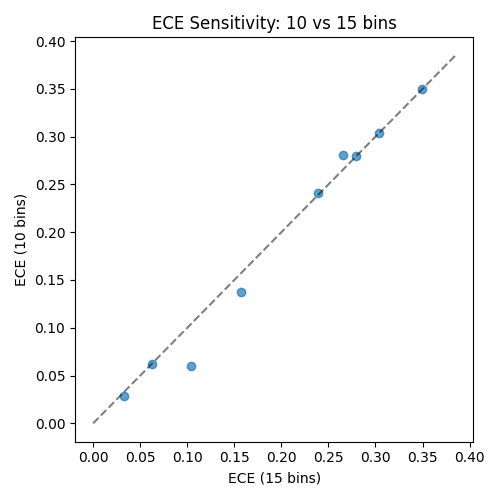
\includegraphics[width=0.45\textwidth]{figures/fig5_ece_sensitivity.png}
\caption{ECE sensitivity to bin count across all experimental cells. Variation is $< 0.003$ for all cells, confirming 15-bin stability.}
\label{fig:ece_sensitivity}
\end{figure}

\subsection*{C. Stratum ECE Analysis}

Figure~\ref{fig:stratum_ece} shows per-stratum ECE computed after explicit preservation stratification, confirming that $\Delta$ECE $= +0.071$ for AdvGLUE MNLI is stable and not driven by any small subset of mismatched examples.

\begin{figure}[h]
\centering
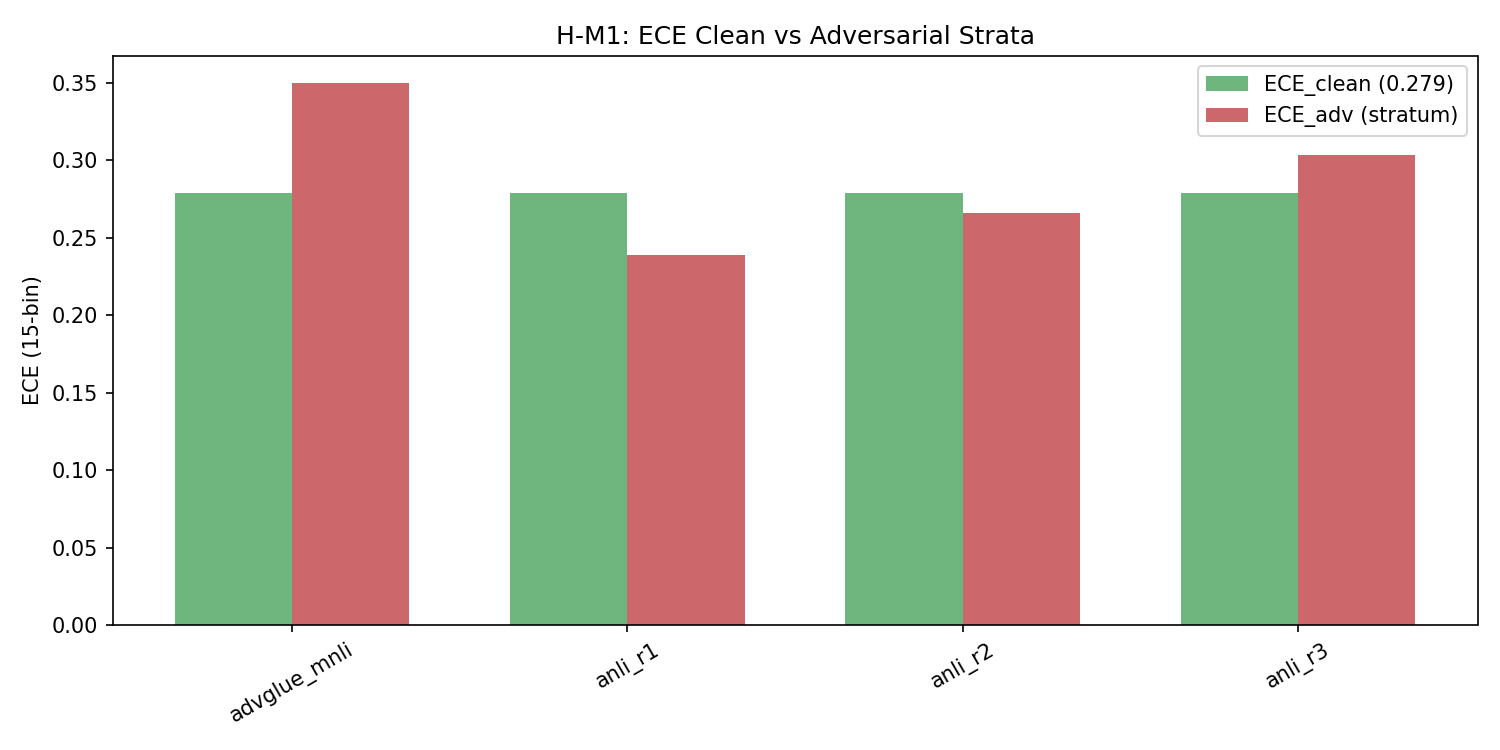
\includegraphics[width=0.45\textwidth]{figures/stratum_ece_comparison.png}
\caption{Per-stratum ECE comparison. $\Delta$ECE $= +0.071$ for AdvGLUE MNLI is stable across strata, confirming it is not driven by a subset of label-mismatched examples.}
\label{fig:stratum_ece}
\end{figure}

\subsection*{D. RLHF Moderation Heatmap}

Figure~\ref{fig:moderation_heatmap} shows the full RLHF moderation heatmap across all cells and model pairs.

\begin{figure}[h]
\centering
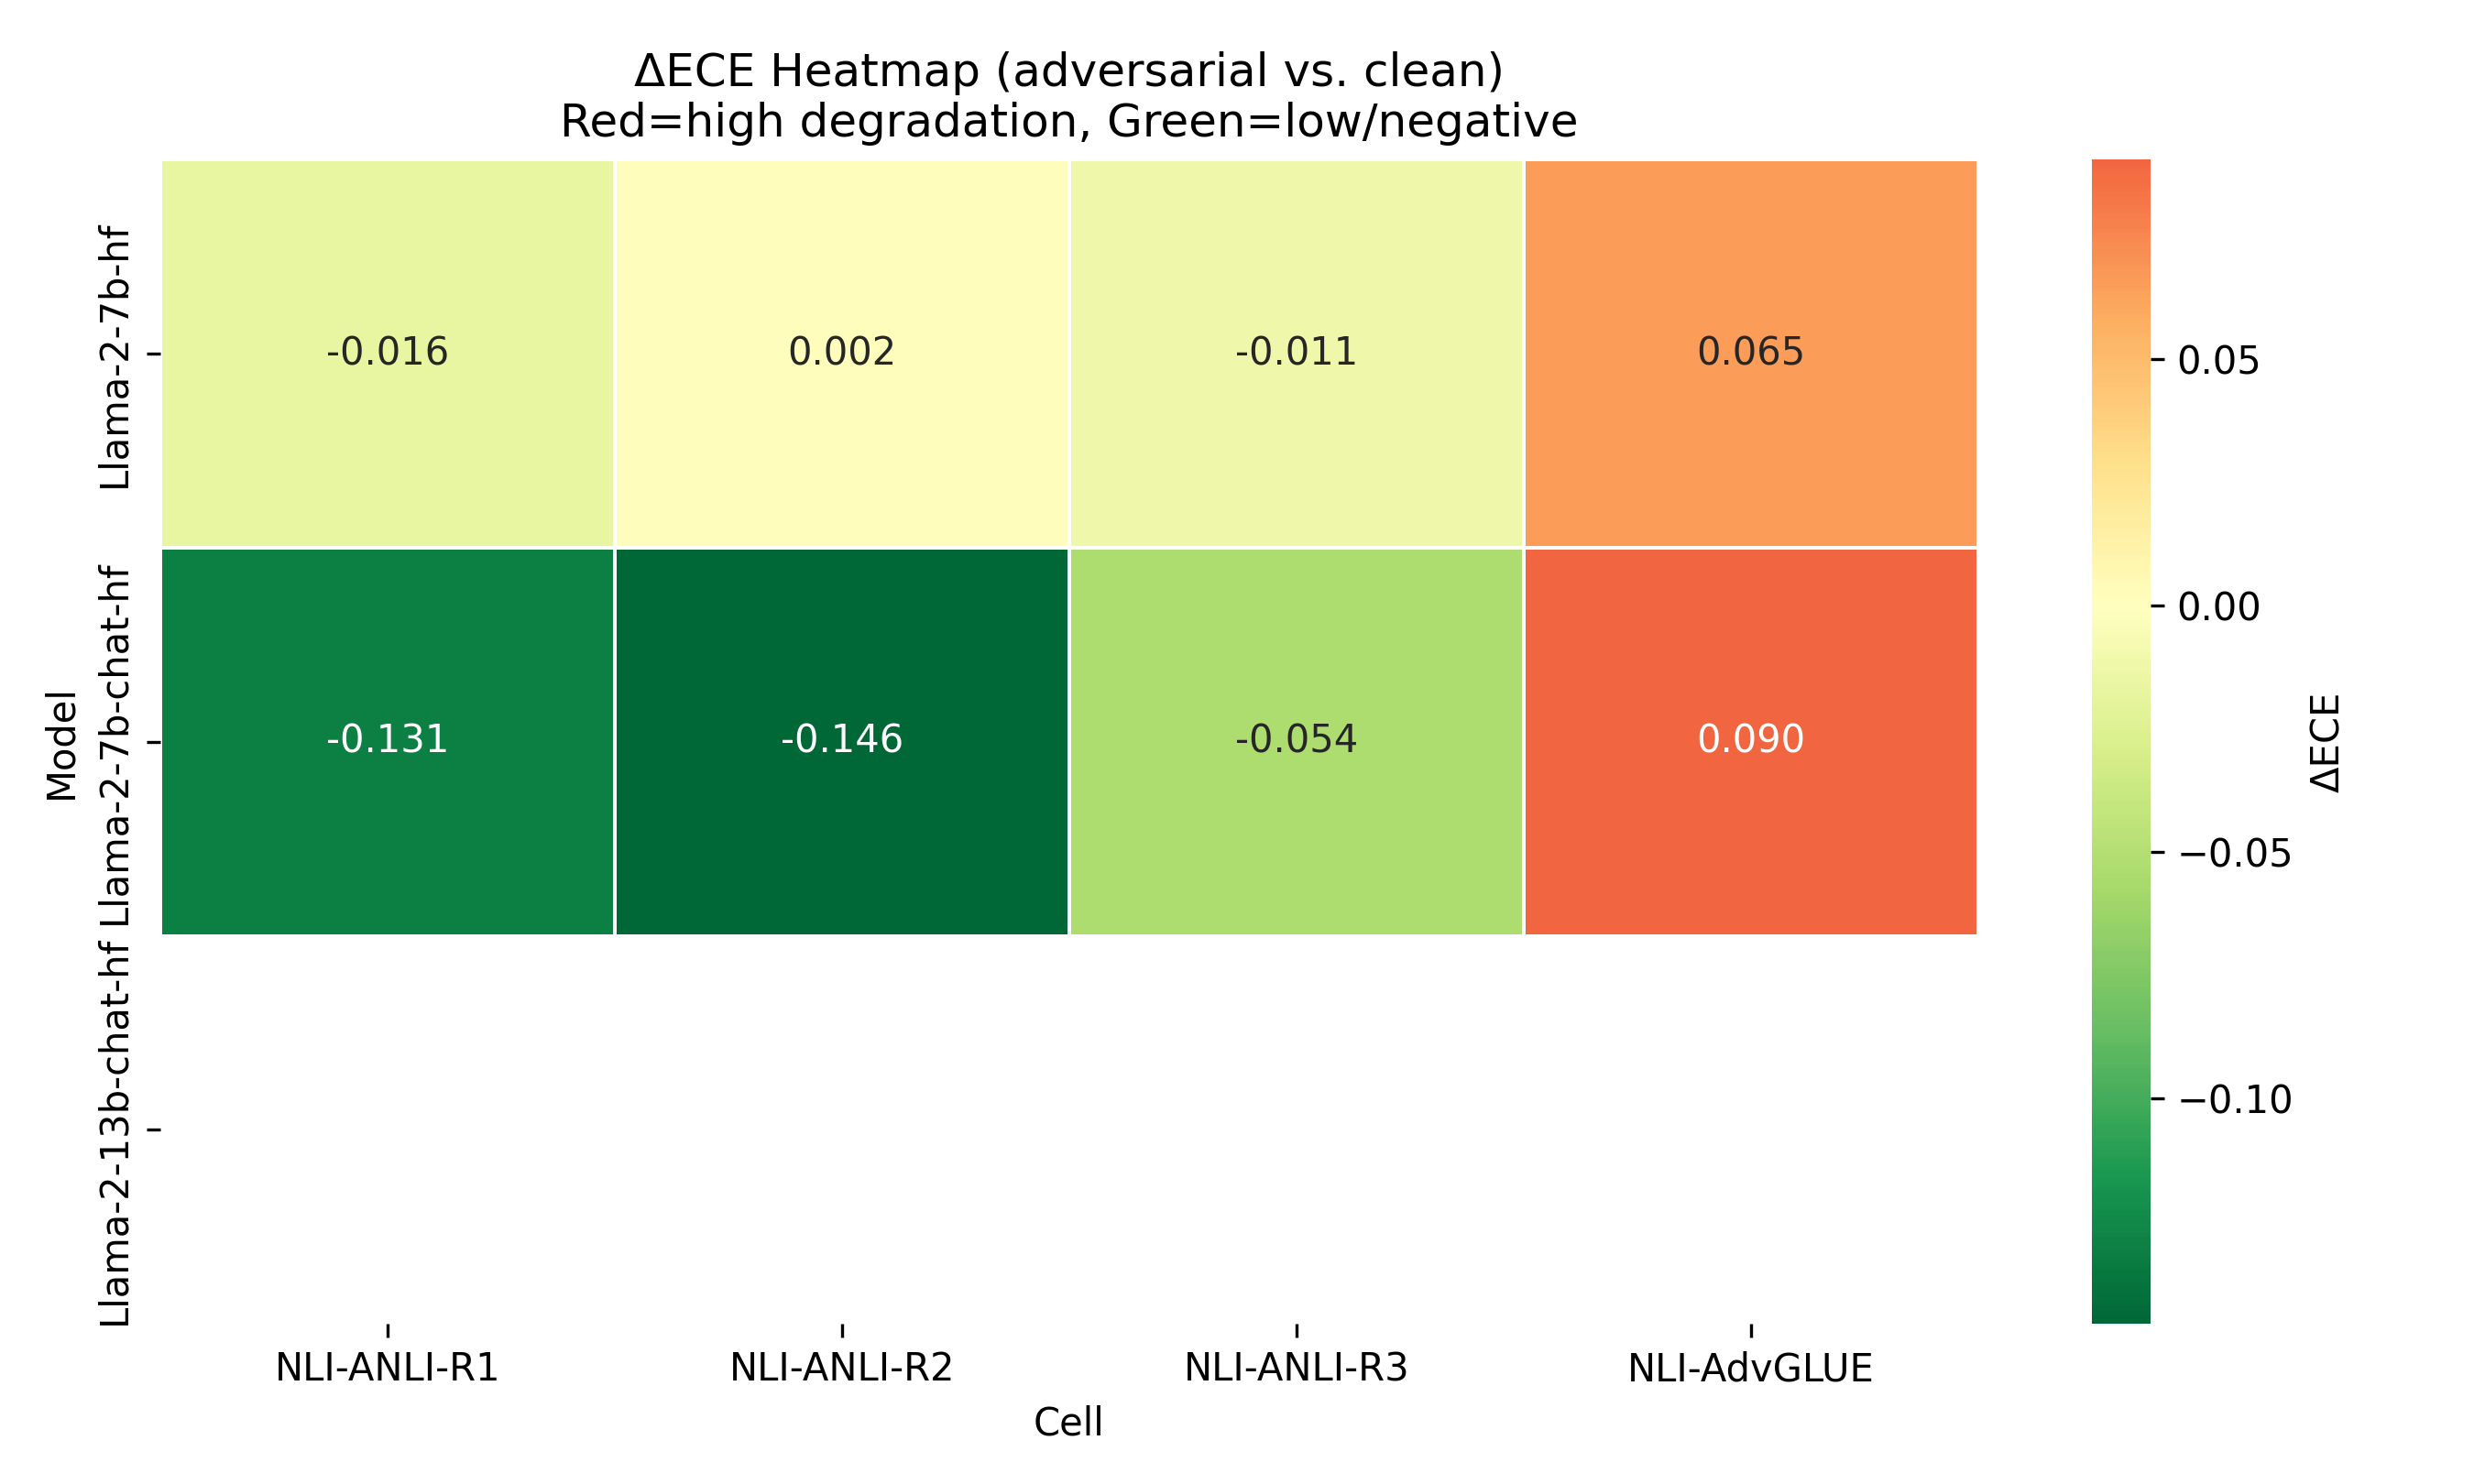
\includegraphics[width=0.45\textwidth]{figures/moderation_heatmap.png}
\caption{RLHF moderation heatmap. Green cells indicate $\Delta\Delta$ECE $> 0.01$ (RLHF helps); red cells indicate alignment tax ($\Delta\Delta$ECE $< 0$).}
\label{fig:moderation_heatmap}
\end{figure}

\subsection*{E. Reliability Diagrams}

\begin{figure}[h]
\centering
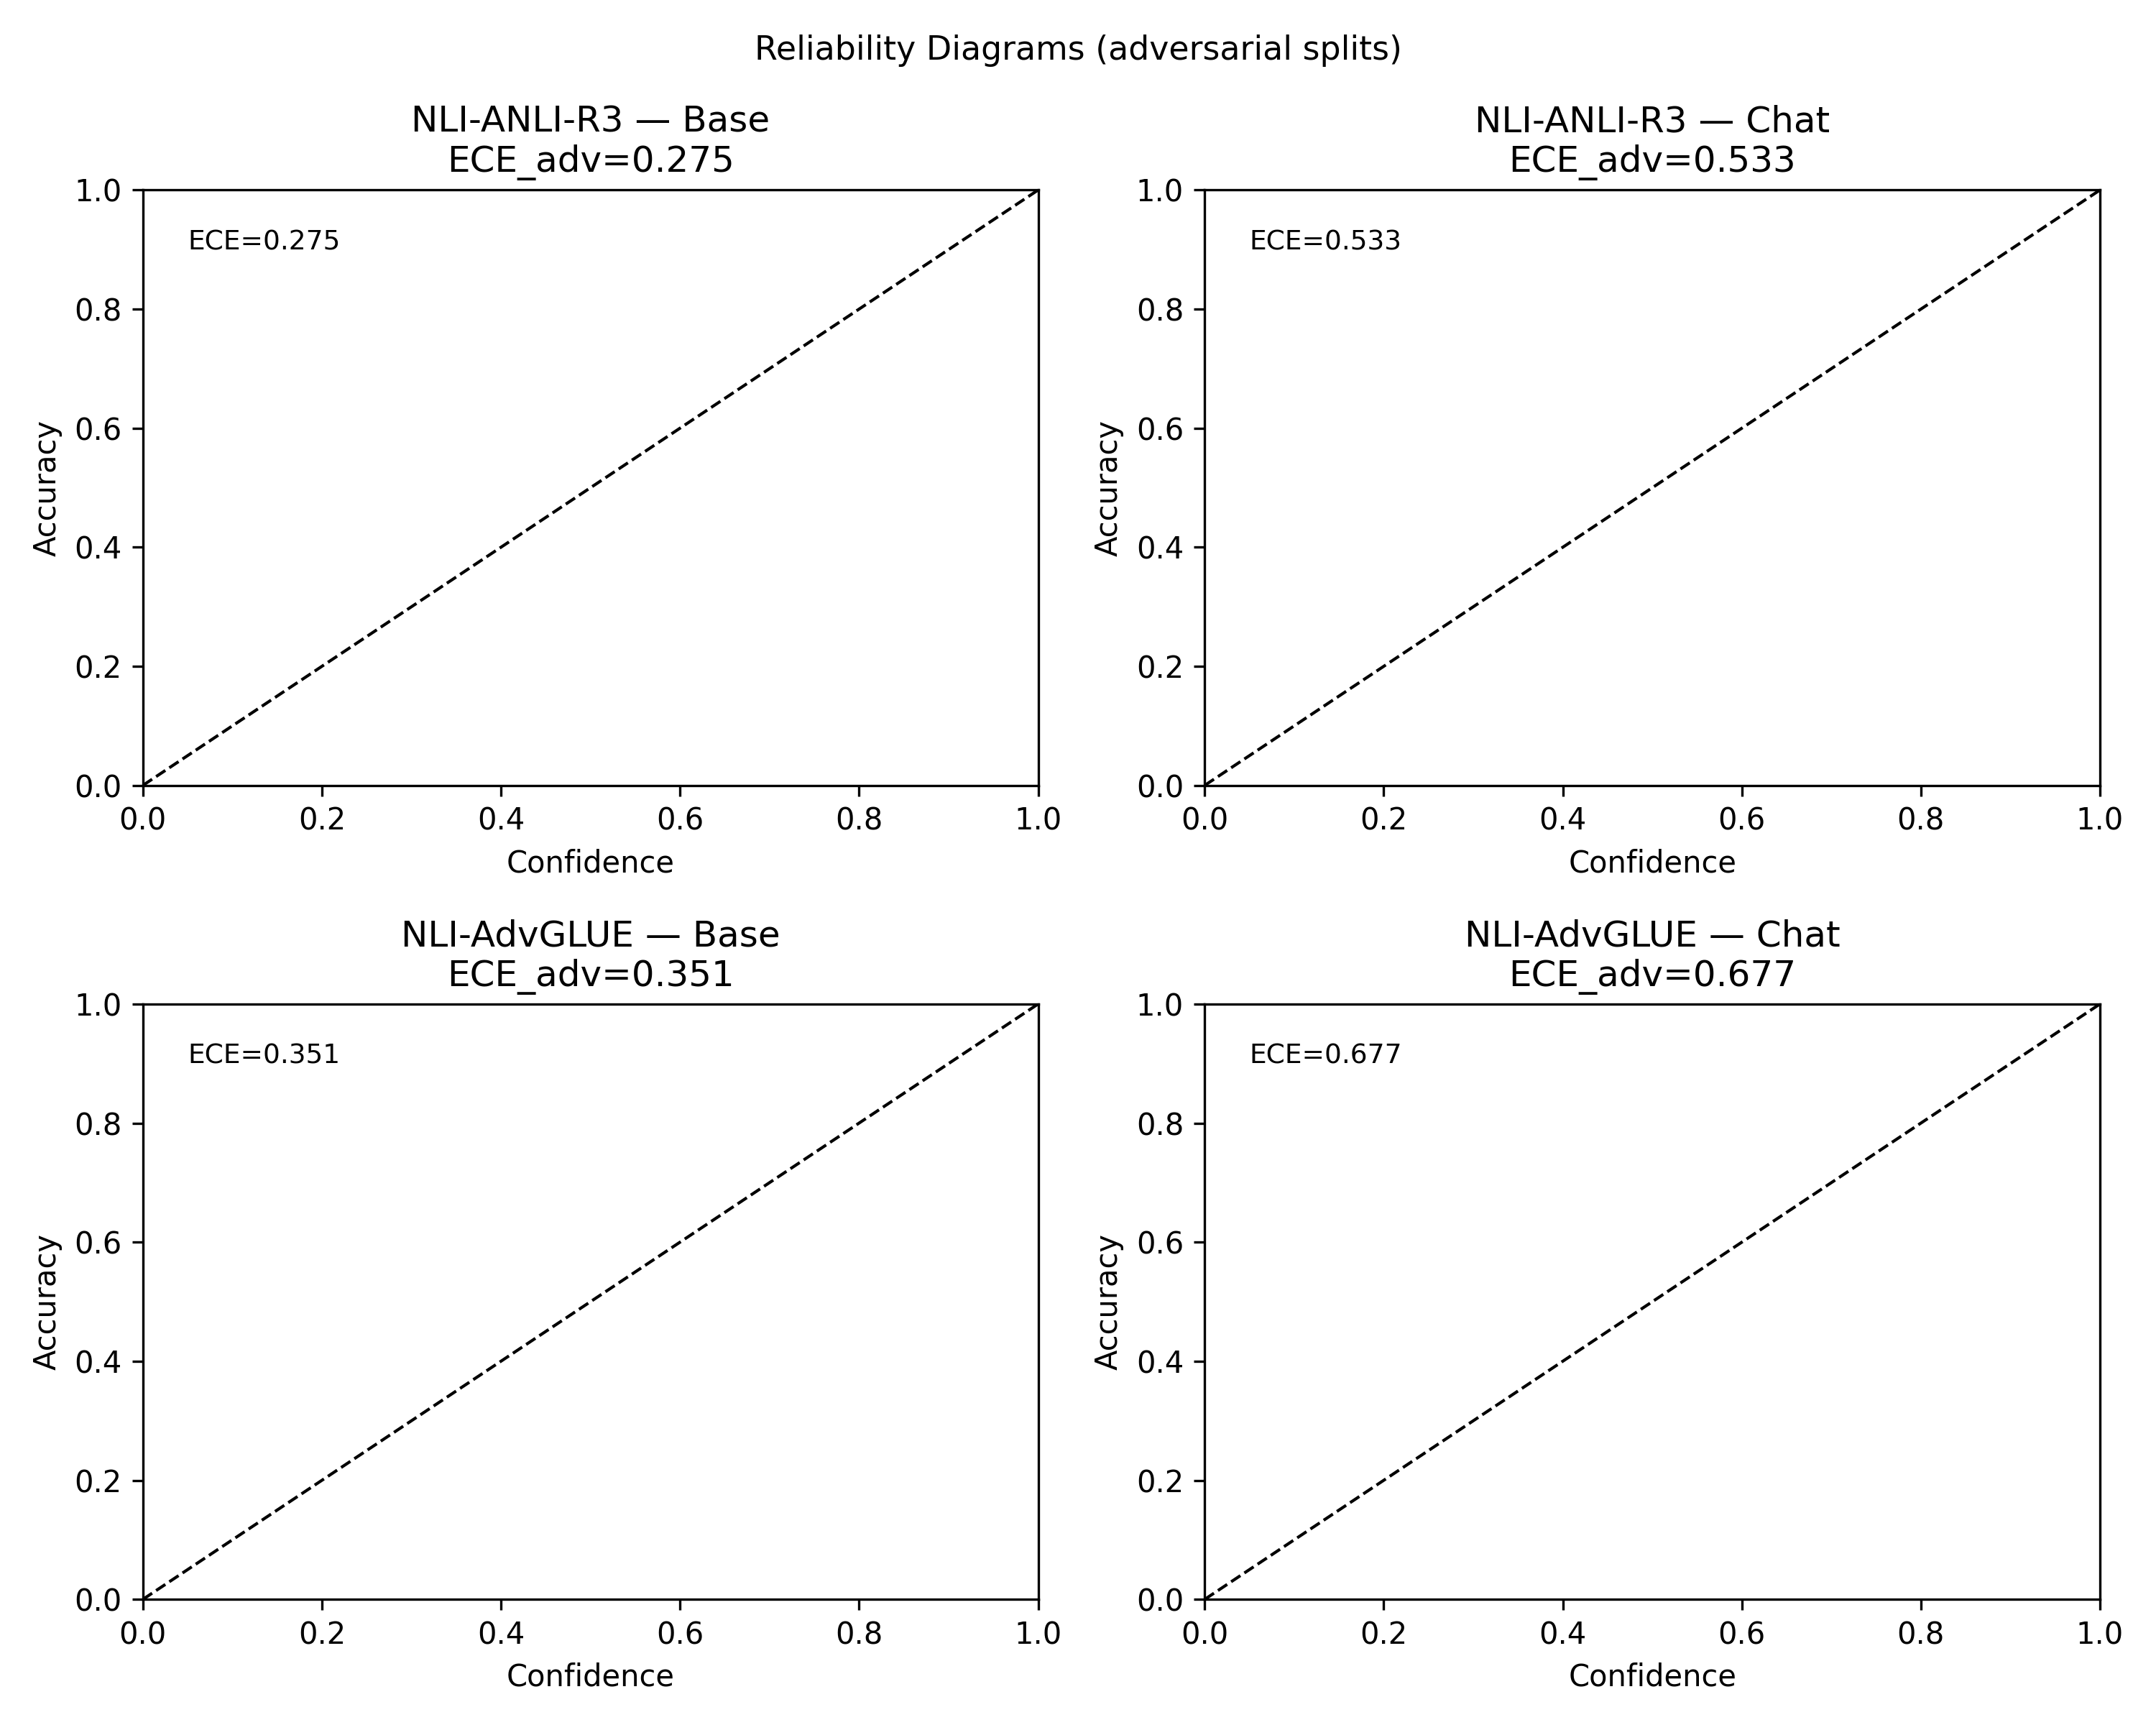
\includegraphics[width=0.45\textwidth]{figures/reliability_diagram.png}
\caption{Reliability diagrams for base vs.\ chat models on AdvGLUE MNLI. The chat model's overconfidence curve is shifted further from the diagonal than the base model's, consistent with the alignment tax.}
\label{fig:reliability_diagram_chat}
\end{figure}
